\documentclass{beamer}
\usepackage[utf8]{inputenc}
\usepackage[slovene]{babel}
\usepackage{amsmath}
\usepackage{mathtools}
\usepackage{multicol}
\usepackage{mathtools}
\renewcommand{\vec}{\underline}
\usetheme{Madrid}
\setbeamertemplate{navigation symbols}{}

\title[Razširjanje zaupanja]{Razširjanje zaupanja za lokalizacijo senzorskih omrežji}
\author[Jaka Velkaverh]{Jaka Velkaverh\\Mentorja: Sergio Cabello, Tomaž Javornik}
\date{26.3.2024}

\theoremstyle{definition}
\newtheorem{definicija}{Definicija}
\newtheorem{izrek}{Izrek}

\begin{document}

  \frame{\titlepage}

  \begin{frame}
    \frametitle{Cilj}
    \begin{block}{Lokalizacija senzorskega omrežja}
      Omrežje si predstavljamo kot utežen graf, kjer so naprave vozlišča.
      Dve vozlišči sta povezani, če sta pripadajoči napravi dovolj blizu,
      da lahko izmerita razdaljo. Utež povezav je izmerjena razdalja,
      kjer pri merjenju pride do napak.

      Vemo lokacije od nekaterih naprav, tem rečemo sidra. Izračunati
      želimo približke za lokacije ostalih, tem rečemo agenti.
    \end{block}
    Predpostavimo, da je omrežje naprav povezano.
  \end{frame}

  \begin{frame}
    \frametitle{Oznake}
    Oznake
    \begin{itemize}
      \item Vozlišča označujemo z črkami $u, v \in V$.
      \item $x_u \in \mathbb{R}^n$ lokacija naprave u.
      \item Za $A = \left\{v_1, v_2, \ldots, v_k\right\} \subseteq V$ je
        $\vec{x}_A = \left(x_{v_1}, x_{v_2}, \ldots, x_{v_k}\right)$
      \item Za $uv \in E$ je $d_{u,v}$ izmerjena razdalja.
    \end{itemize}
  \end{frame}

  \begin{frame}
    $$E\left(\vec{x}_V\right) \coloneqq \sum_{uv \in E}\left(\left|x_u - x_v\right|-d_{u,v}\right)^2$$
    \pause
    $$P\left(\vec{x}_V\right) \coloneqq exp\left[-\sum_{uv \in E}\left(\left|x_u - x_v\right|-d_{u,v}\right)^2\right] =
    \prod_{uv \in E}e^{-\left(\left|x_u - x_v\right|-d_{u,v}\right)^2}$$
    $$
    = \prod_{uv \in E}\psi_{u,v}\left(x_u,x_v\right)
    $$
    \pause
    Omejimo na $S \subseteq \mathbb{R}^{n\cdot \left|V\right|}$ s končnim volumnom.
    $$\tilde{P}\left(\vec{x}_V\right) \coloneqq \left(\int_S P\left(\vec{z}_V\right)d\vec{z}_V\right)^{-1}
    P\left(\vec{x}_V\right)$$
    \pause
    $\vec{X}_V$ zvezno porazdeljen slučajni vektor z gosto $\tilde{P}$.
  \end{frame}

  \note{
    Najprej definiramo t.i.\ funkcijo energije $E$, ki predvidenim lokacijam
    naprav predpiše pozitivno število, ki je majhno, če so medsebojne razdalje
    blizu predvidenim. Smiselno bi bilo proglasiti predvidene lege kot tiste,
    ki minimizerajo to funkcijo.

    Nato funkcijo energije komponiramo s padajočo funkcijo $e^{-x}$, da dobimo
    funkcijo $P$ z vrednostmi v $(0, 1]$. Če smo funkcijo $E$ minimizerali,
    bomo funkcijo $P$ maksimizirali. Če se z vrednostmi $\vec{x}_V$ omejimo,
    jo lahko še normaliziramo. Tako lahko z njo kot gostoto definiramo slučajni
    vektor $\vec{X}_V$. Iščemo torej najbolj verjetno lego slučajnega vektorja
    $\vec{X}_V$.
  }

  \begin{frame}
    \frametitle{Markovska polja}
    \begin{block}{Pogojna neodvisnost}
      Nakjučna vektorja $\vec{X}, \vec{Y}$ sta pogojno
      neodvisna ob $\vec{Z}$, če velja:
      $$f_{\vec{X}, \vec{Y}|\vec{Z}}\left(\vec{x}, \vec{y}\ |\ \vec{Z} = \vec{z}\right) =
      f_{\vec{X}|\vec{Z}}\left(\vec{x}\ |\ \vec{Z} = \vec{z}\right) \
      f_{\vec{Y}|\vec{Z}}\left(\vec{y}\ |\ \vec{Z} = \vec{z}\right)
      $$
    \end{block}
    \pause
    \begin{definicija}
      Graf $G = \left(V, E\right)$, in slučajne spremenljivke
      $\vec{X}_V$ tvorijo Markovsko polje,
      če velja Markovska lastnost po parih:

      Za vsaka nesosedna $u, v \in V$ sta $X_u$, $X_v$
      pogojno neodvisna ob vseh ostalih
      $\vec{X}_{V\backslash\left\{u, v\right\}}$
    \end{definicija}
  \end{frame}

  \begin{frame}
    \frametitle{$\vec{X}_V$ je Markovsko polje}
    Za nesosednja $u, v \in V$ je
    $$
    f_{X_u,X_v|\vec{X}_{V\backslash \left\{u,v\right\}}}
      \left(x_u,x_v | \vec{X}_{V\backslash \left\{u,v\right\}} = \vec{y}_{V\backslash \left\{u,v\right\}}\right) \propto
    $$
    \pause
    $$
    \propto \prod_{su \in E}\psi_{s,u}\left(y_s,x_u\right)
      \prod_{sv \in E}\psi_{s,v}\left(y_s,x_v\right)
      \prod_{\substack{\left\{s,t\right\} \in E \\ \left\{s,t\right\}\cap \left\{u,v\right\} = \emptyset}}\psi_{s,v}\left(y_s,y_t\right)
      \propto
    $$
    \pause
    $$
    \propto g\left(x_u\right) h\left(x_v\right) \Rightarrow X_u, X_v \text{ pogojno neodvisna ob } \vec{X}_{V\backslash \left\{u,v\right\}}
    $$
  \end{frame}

  \note{
    Tu pokažem, da gostota $\vec{X}_V$ zadošča Markovski lastnosti po parih.

    V prejšnji predstavitvi sem se tu skliceval na Hammersley-Cliffordov izrek,
    ampak sem šel to raje dokazal direktno, ker je tu precej nepotreben.
  }

  \begin{frame}
    \frametitle{Razširjanje zaupanja na drevesih}
    Poglejmo si primer, ko je graf drevo.
    \setlength{\columnsep}{-5cm}
    \begin{multicols}{2}
      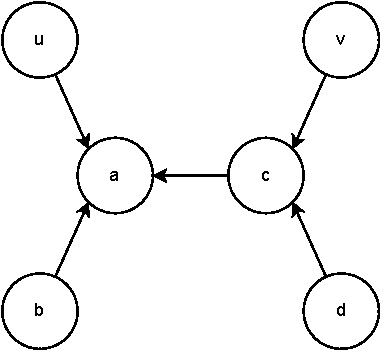
\includegraphics[width=4cm]{message_passing.pdf}
      \columnbreak{}

      \vspace{5cm}
      $$
      \int_{\vec{X}_{V_a \backslash \left\{a\right\}}} f_{\vec{X}_{V_a} | \vec{X}_{V_s}}\left(\vec{x}_{V_a} | \vec{x}_{V_s} = \vec{y}_{V_s}\right)
      d\vec{x}_{V_a \backslash \left\{A\right\}}\propto
      $$
      $$
      \quad \int_{X_b,X_d,X_c} \psi_{u,a} \psi_{b,a} \psi_{c,a} \psi_{v,c} \psi_{d,c}dx_bdx_ddx_c =
      $$
      \pause
      \vspace{1cm}
      $$
      \psi_{u,a} \int_{X_b} \psi_{b,a}dx_b \int_{X_c} \psi_{c,a} \psi_{v,c}
      \int_{X_d} \psi_{d,c}dx_ddx_c
      $$
    \end{multicols}
  \end{frame}

  \note{
  	Ta primer je enak kot na kratki predstavitvi.
  }

  \begin{frame}
    \begin{align*}
      \text{Za } u,v \in V_a\text{: } &
      \mu_{u \to v}\left(x_v\right) \coloneqq
      \int_{X_u} \psi_{u,v}\left(x_u,x_v\right)
      \prod_{t\in N\left(u\right)\backslash v}
      \mu_{t \to u}\left(x_u\right)dx_u
      \\
      \text{Za }u \in V_s\text{ in }v \in V_a\text{: } &
      \mu_{u \to v}\left(x_v\right) \coloneqq
      \psi_{u,v}\left(y_u,x_v\right)
    \end{align*}
    \pause
    $$
    \Rightarrow
    \psi_{u,a} \int_{X_b} \psi_{b,a}dx_b \int_{X_c} \psi_{c,a} \psi_{v,c}
    \int_{X_d} \psi_{d,c}dx_ddx_c=
    $$
    \pause
    $$
    \mu_{u \to a}\left(x_a\right)\mu_{b \to a}\left(x_a\right)
    \int_{X_c} \psi_{c,a}
    \mu_{v \to c}\left(x_c\right)
    \mu_{d \to c}\left(x_c\right)dx_c=
    $$
    \pause
    $$
    \mu_{u \to a}\left(x_a\right)\mu_{b \to a}\left(x_a\right)
    \mu_{c \to a}\left(x_a\right) =
    $$
    $$
    \prod_{t \in N\left(a\right)}\mu_{t \to a}\left(x_a\right) \eqqcolon M_a\left(x_a\right)
    $$
  \end{frame}

  \begin{frame}
    \frametitle{Pravilnost razširjanja zaupanja na drevesih}
    \begin{izrek}
      Naj bo $G = \left(V, E\right)$ drevo in $V_a$, $V_s$, $\vec{X}_V$,
      $\vec{y}_{V_s}$, $M_u\left(x_u\right)$ kot prej.
      Zaupanje je proporcionalno robni gostoti
      $$
      M_u\left(x_u\right) \propto f_{X_u | \vec{X}_{V_s}}\left(x_u | \vec{X}_{V_s} = \vec{y}_{V_s}\right).
      $$
    \end{izrek}
    Ideja dokaza so poddrevesa osnovnega drevesa s korenom v $u$.
  \end{frame}

  \note{
  	Ker so sporočila definirana rekurzivno, se je treba najprej prepričati, da
  	obstaja vrstni izračuna, v katerem imamo na vsakem koraku že izračunana
  	vsa potrebna sporočila za izračun trenutnega sporočila. Za drevesa to velja,
  	kar bom na predstavitvi pokazal z indukcijo.

  	Po tem lahko dokažem še trditev iz prosojnice.
  }

  \begin{frame}
    \frametitle{Za grafe s cikli}
    Naj bosta $u,v \in V_a$, $i \in \mathbb{N}$ pa število iteracije.
    $$
    M_u^{\left(i\right)}\left(x_u\right) \coloneqq
    \prod_{t \in N\left(u\right)}\mu^{\left(i\right)}_{t \to u}\left(x_u\right)
    $$
    $$
    \mu_{v \to u}^{\left(i\right)}\left(x_u\right) \coloneqq
    \int_{X_v} \psi_{v,u}\left(x_v,x_u\right)
    \frac{
      M_v^{\left(i-1\right)}\left(x_v\right)}{
      \mu_{u \to v}^{\left(i-1\right)}\left(x_v\right)
    }dx_v
    $$
    Za $v \in V_s$, $u \in V_a$ je pa
    $\mu_{v \to u}^{\left(i\right)}\left(x_u\right) \coloneqq \psi_{v,u}\left(y_v, x_u\right)$

    Za drevesa to konvergira k pravim vrednostim.
  \end{frame}

  \note{
  	Konvergence ne bom dokazal.

  	Ta slide je enak kot na kratki predstavitvi.
  }

  \begin{frame}
    \frametitle{Izboljšave}
    \begin{itemize}
      \item Za $u,v$, ki $d\left(u,v\right) \geq 2$, dodamo potenciale.
      \item Potenciale popravimo zaradi velikih odstopanj.
      \item Sporočilo $\mu_{u \to v}$ aproksimiramo z
        $\sum_{i=1}^{n}\frac{w_i}{\sqrt{2\pi}} exp\left[-\frac{\left|x-x_i\right|^2}{2\sigma_i^2}\right]$.
      \item Algoritem izvajamo večkrat na vpetih drevesih.
    \end{itemize}
  \end{frame}

  \note{
  	Pri prem za $u,v$ vemo, da nista izmerila medsebojne razdalje in iz tega
  	sklepamo, da nista blizu skupaj. Na podlagi tega lahko dodamo potencial,
  	ki narašča z razdaljo. Za nek $R > 0$ lahko izberemo
  	$$\psi_{u,v}\left(x_u,x_v\right) =
  	\begin{cases}
  		1 & \text{; } \left|x_u - x_v\right| \geq R\\
  		0 & \text{; } \left|x_u - x_v\right| < R
  	\end{cases}
  	$$
  	ali pa raje $\psi_{u,v}\left(x_u,x_v\right) =
  	1 - exp\left[-\frac{\left|x_u-x_v\right|^2}{2R^2}\right]$.

  	Pri drugem za potenciale dodamo neko konstanto, da potenciali
  	ob $x_u$, $x_v$, katerih razdalja je močno različna od $d_{u,v}$ ne zavzamejo
  	premajhnih vrednosti. V praksi se izkaže, da če tega ne naredimo, je
  	lokalizacija zelo občutljiva na veliko meritveno napako pri le eni razdalji.
  }

  \note{
  	Tretja točka govori o \emph{nonparametric belief propagation}.

  	Pri četrti točki bo gotovo algoritem na vsakem vpetem
  	drevesu konvergiral, a pri vsakem od rezultatov upošteva le nekatere povezave.
  	Na koncu zaupanje za vozlišče dobimo tako, da zmnožimo zaupanja tega vozlišča
  	iz vseh dreves. V praksi to deluje dobro za goste grafe.
  }

\end{document}

